\documentclass[a4paper]{article}
\usepackage{import}
\usepackage[utf8]{inputenc}
\usepackage[T1]{fontenc}
\usepackage{textcomp}
\usepackage[italian]{babel}
\usepackage{amsmath, amssymb}
\usepackage{booktabs,xltabular}
\usepackage{amsfonts}
\usepackage{subcaption}
\usepackage{amsthm}
\usepackage{cancel}
\usepackage{mdframed}
\usepackage{makecell}
\usepackage{float}
\usepackage{xcolor}
\usepackage{listings}
\usepackage{gensymb}
\usepackage{graphicx}
\usepackage{bodeplot}
\usepackage{physics}
\usepackage{tikz}
\usetikzlibrary{shapes, arrows, automata, petri, decorations.markings, decorations.pathreplacing, positioning, calc, quotes}
\usepackage{circuitikz}
\usepackage[label=corner]{karnaugh-map}
\graphicspath{{./figures/}}

% Set default font to sans-serif
\renewcommand{\familydefault}{\sfdefault} 
\usepackage{eulervm}

\usepackage{forest}

\usepackage{mathtools}
\DeclarePairedDelimiter\ceil{\lceil}{\rceil}
\DeclarePairedDelimiter\floor{\lfloor}{\rfloor}

% \usepackage{ntheorem}

\usepackage{import}
\usepackage{pdfpages}
\usepackage{transparent}
\usepackage{xcolor}

\usepackage{hyperref}
\hypersetup{
    colorlinks=false,
}

% Code blocks
\definecolor{codegreen}{rgb}{0,0.6,0}
\definecolor{codegray}{rgb}{0.5,0.5,0.5}
\definecolor{codepurple}{rgb}{0.58,0,0.82}
\definecolor{backcolour}{rgb}{0.95,0.95,0.95}

\lstdefinestyle{mystyle}{
	backgroundcolor=\color{backcolour},
	commentstyle=\color{codegreen},
	keywordstyle=\color{magenta},
	numberstyle=\tiny\color{codegray},
	stringstyle=\color{codepurple},
	basicstyle=\ttfamily\footnotesize,
	breakatwhitespace=false,
	breaklines=true,
	captionpos=b,
	keepspaces=true,
	numbers=left,
	numbersep=5pt,
	showspaces=false,
	showstringspaces=false,
	showtabs=false,
	tabsize=2
}

\lstset{style=mystyle}

\usepackage{color}
\usepackage{import}
\usepackage{pdfpages}
\usepackage{transparent}
\usepackage{xcolor}

% Example frame
\theoremstyle{definition}
\newmdtheoremenv[%
	linecolor=gray,leftmargin=0,%
	rightmargin=0,
	innertopmargin=8pt,%
	innerbottommargin=8pt,
	ntheorem]{example}{Esempio}[section]

% Important definition frame
\theoremstyle{definition}
\newmdtheoremenv[%
	linecolor=gray,leftmargin=0,%
	rightmargin=0,
	backgroundcolor=gray!40,%
	innertopmargin=8pt,%
	innerbottommargin=8pt,
	ntheorem]{definition}{Definizione}[section]

% Exercise frame
\theoremstyle{definition}
\newmdtheoremenv[%
	linecolor=gray,leftmargin=0,%
	rightmargin=0,
	innertopmargin=8pt,%
	innerbottommargin=8pt,
	ntheorem]{exercise}{Esercizio}[section]

% Theorem frame
\theoremstyle{definition}
\newmdtheoremenv[%
  linecolor=gray,leftmargin=0,%
  rightmargin=0,
  innertopmargin=8pt,%
  innerbottommargin=8pt,
  ntheorem]{theorem}{Teorema}[section]

\theoremstyle{definition}
\newmdtheoremenv[%
  linecolor=white,leftmargin=0,%
  rightmargin=0,
  innertopmargin=8pt,%
  innerbottommargin=8pt,
  ntheorem]{define}{Definizione utile}[section]

% figure support
\usepackage{import}
\usepackage{xifthen}
\pdfminorversion=7
\usepackage{pdfpages}
\usepackage{transparent}
\newcommand{\incfig}[1]{%
	\def\svgwidth{\columnwidth}
	\import{./figures/}{#1.pdf_tex}
}

% FSM tikz
\tikzset{
    place/.style={
        circle,
        thick,
        draw=black,
        minimum size=6mm,
    },
        state/.style={
        circle,
        thick,
        draw=black,
        fill=white,
        minimum size=6mm,
    },
}

\pdfsuppresswarningpagegroup=1

\usepackage{pgfplots}
\pgfplotsset{compat=1.18,width=10cm}

% Save plots as pdf and reuse them without compiling every time
\usetikzlibrary{external}
\tikzexternalize[prefix=figures/tikz/, optimize=false]


% Libro: Sakurai

% Potenziali approfondimenti:
% Qiskit: implementare un circuito di teletrasporto
% E collegarsi a computer quantistico di IBM
% Quantum machine learning (lettura di un paper)
% Approfondire le altre porte (teletrasporto)
\begin{document}

\begin{titlepage}
	\begin{center}
		\vspace*{1cm}

		\Huge
		\textbf{Probabilità e Statistica\\Esercizi}

		\vspace{0.5cm}
		\LARGE
		UniVR - Dipartimento di Informatica

		\vspace{1.5cm}

		\textbf{Fabio Irimie}

		\vfill


		\vspace{0.8cm}


		2° Semestre 2023/2024

	\end{center}
\end{titlepage}


\tableofcontents
\pagebreak

\section{Formalismo della meccanica quantistica}
Deriviamo il formalismo partendo dall'esperimento di Stern-Gerlach e di Feynman utilizzando la
notazione di Dirac.

\subsection{Principi}
\begin{itemize}
  \item Ad un \textbf{sistema fisico} corrisponde uno spazio vettoriale complesso
    di dimensione \( n \), dove \( n \) è il numero di gradi di libertà del sistema
    quanto-meccanico. Il grado di libertà è il numero di alternative, o scelte, a
    disposizione del sistema (da qui deriva il termine "quantistico", siccome le
    alternative sono quantizzate).
    \[
    \text{Sistema fisico } \to \mathbb{C}^n
    \] 

    \vspace{1em}
    \noindent
    Ad esempio nell'espermimento di Stern-Gerlach la misura è lo spin di un atomo
    che può avere solo due valori, quindi \( \pm \frac{\hslash}{2} \), ovvero \( n = 2 \).

    Nell'esperimento di Feynman con la doppia fenditura il sistema è una particella
    che può passare per una delle due fenditure, quindi \( n = 2 \).
    Se oltre al percorso in cui è passato l'atomo si vuole sapere anche lo spin, allora
    il grado di libertà aumenta.

    \vspace{1em}
    \noindent
    I sistemi con \( n = 2 \) si chiamano \textbf{sistemi a due stati}.

  \item Allo \textbf{stato fisico} corrisponde un vettore di stato dello spazio 
    vettoriale complesso chiamato \textbf{Ket}. Nella notazione di Dirac il vettore di
    stato è indicato con \( \ket{\alpha} \). Questo vettore è definito a meno di una 
    costante, quindi:
    \[
      \ket{\alpha} \iff c \ket{\alpha}
    \] 
    sono lo stesso stato e ciò significa che il Ket è \textbf{normalizzato} e sarà un 
    vettore unitario.

    \vspace{1em}
    \noindent
    Ad esempio un atomo di argento con un certo spin rappresenta uno stato fisico. E
    il Ket contiene tutte le informazioni riguardanti alla direzione (""raggi"") che si possono 
    avere su quell'atomo.

  \item Un \textbf{osservabile} è una variabile fisica che si può misurare. All'osservabile
    corrisponde un operatore dello spazio \( \mathbb{C}^n \) che agisce sui Ket e
    restituisce un altro Ket:
    \[
      \mathcal{A} \ket{\alpha} \quad \text{dove } \mathcal{A} \text{ è l'operatore che
      agisce su alfa}
    \] 
    (potrebbero essere matrici se si trova una base ad esempio)

    \vspace{1em}
    \noindent
    Ci sono degli operatori importanti, cioè quelli che agendo su un Ket \( \ket{a_i} \)
    restituiscono un vettore parallelo ad \( \ket{a_i} \) e quindi sono \textbf{autoKet}
    (si può pensare agli autovettori dell'algebra linare):
    \[
      \underbrace{\mathcal{A} \ket{a_i}}_{\text{autoKet } \leftrightarrow \text{ autostato}}
      = \underbrace{a_i}_{\text{autovalore}} \ket{a_i}
    \] 
    L'oggetto risultante rappresenta lo stesso stato fisico, siccome è solo moltiplicato
    per una costante. L'insieme degli autoKet e autostati è rappresentato come:
    \[
      \left\{ \ket{a_i} \right\}; \left\{ a_i \right\}
    \] 

    \vspace{1em}
    \noindent
    Ad esempio nell'esperimento di Stern-Gerlach si aveva l'operatore
    \( \mathcal{S}_{\hat{z}} \) che rappresentava la misura dello spin lungo l'asse \( z \).
    \[
      \left\{ \mathcal{S}_z; \pm \right\}; \left\{ \pm \frac{\hslash}{2} \right\}
    \] 
    nell'esperimento si ha che l'operatore \( \mathcal{S}_z \) che agisce sullo stato a
    spin in su restituisce:
    \[
      \mathcal{S}_z \ket{\mathcal{S}_z; +} = \frac{\hslash}{2} \ket{\mathcal{S}_z; +}
    \] 
    l'operatore \( \mathcal{S}_z \) agisce sullo stato a spin in giu restituisce:
    \[
      \mathcal{S}_z \ket{\mathcal{S}_z; -} = -\frac{\hslash}{2} \ket{\mathcal{S}_z; -}
    \]

    \vspace{1em}
    \noindent
    Nell'esperimento di Stern-Gerlach i due autoKet di \( \mathcal{S}_z \) sono una base
    dello spazio \( \mathbb{C}^2 \) e quindi si può scrivere un qualsiasi Ket come
    combinazione lineare di questi due Ket:
    \[
      \begin{aligned}
        \ket{\mathcal{S}_x; \pm}\\
        \ket{\mathcal{S}_y; \pm}\\
      \end{aligned}
    \] 
    Un generico stato rappresentato come combinazione lineare di questi Ket è:
    \[
      \ket{\alpha} = c_+ \ket{\mathcal{S}_z; +} + c_- \ket{\mathcal{S}_z; -}
    \] 
    o anche la seguente notazione (qbit):
    \[
      \ket{\alpha} = c_0 \ket{0} + c_1 \ket{1}
    \] 

  \item Qualsiasi \textbf{generico stato fisico} del sistema si può rappresentare come 
    \textbf{sovrapposizione di autostati}, cioè una combinazione lineare degli autoKet.
    \[
      \ket{\alpha} = \sum_i^n c_i \ket{a_i}
    \] 
    (questo sviluppo è unico per il sistema \( a_i \))
    dove \( n \) è il grado di libertà e:
    \[
      A \ket{a_i} = a_i \ket{a_i}
    \] 
    Finchè non viene effettuata una misura, il sistema è in uno stato di sovrapposizione
    e non si può sapere il suo stato.
    \vspace{1em}
    \noindent
    Trovare tutti gli autostati di un sistema si chiama problema di quantizzazione.
\end{itemize}

\subsection{Operazioni}
\subsubsection{Prodotto "interno"}
\begin{itemize}
  \item Esiste una corrispondenza uno ad uno tra lo spazio degli stati (Ket) e un suo
    spazio duale (Bra):
    \[
      \underset{\text{Ket}}{\ket{\alpha}} \stackrel{\text{Duale}}{\longleftrightarrow} 
      \underset{\text{Bra}}{\bra{\alpha}}
    \] 

    La base dei Ket è in corrispondenza duale con la base dei Bra:
    \[
      \underbrace{\{\ket{a_n}\}}_{\text{autoKet}} \stackrel{\text{C.D.}}{\longleftrightarrow}
      \underbrace{\{\bra{a_n}\}}_{\text{autoBra}}
    \]
    ad exempio:
    \[
      C \ket{\alpha} \stackrel{\text{C.D.}}{\longleftrightarrow} C^* \bra{\alpha}
    \] 
    dove \( C^* \) è il complesso coniugato di \( C \). Questo vuol dire che ad una
    somma di Ket corrisponde la somma dei Bra.
\end{itemize}
Vogliamo definire un prodotto tra stati fisici.
\begin{definition}[Prodotto interno]
  È definito \textbf{prodotto interno} il prodotto tra un Ket e un Bra:
  \[
    \underbrace{\braket{\alpha}{\beta}}_{\text{Notazione di Dirac}} = \left(\bra{\alpha}\right) \cdot \left(\ket{\beta}\right)
  \] 
\end{definition}

\vspace{1em}
\noindent
\textbf{Proprietà}:

\begin{itemize}
  \item \( \braket{\alpha}{\beta} = \braket{\beta}{\alpha}^* \) 
  \item \( \braket{\alpha}{\alpha} \geq 0 \), quindi \( \braket{\alpha}{\alpha} \) è reale.
\end{itemize}

\begin{definition}[Ket ortogonali]
  Due Ket sono \textbf{ortogonali} quando:
  \[
    \braket{\alpha}{\beta} = 0
  \] 
\end{definition}

\vspace{3em}
\noindent
Con questo operatore si possono normalizzare gli stati fisici, che sono definiti a meno di
una costante.
\begin{definition}[Normalizzazione]
  La normalizzazione di uno stato fisico si esegue come:
  \[
    \ket{\hat{\alpha}} = \frac{\ket{\alpha}}{\sqrt{\braket{\alpha}{\alpha}}}
  \] 

  \vspace{1em}
  \noindent
  Di conseguenza
  \[
    \braket{\hat{\alpha}}{\hat{\alpha}} = 1
  \] 
\end{definition}

\subsubsection{Operazioni illecite}
Alcune operazioni nella meccanica quantistica sono vietate, perchè non hanno significato.
\begin{itemize}
  \item Un operatore non può agire su un Ket da destra:
    \[
      \begin{aligned}
        A \ket{\alpha} \quad \color{green}\surd\\
        \ket{\alpha}A \quad \color{red}\times
      \end{aligned}
    \] 
    Analogamente un osservabile non può agire da sinistra su un Bra:
    \[
      \begin{aligned}
        \bra{\alpha}A \quad \color{green}\surd\\
        A\bra{\alpha} \quad \color{red}\times
      \end{aligned}
    \]

  \item Non ha significato moltiplicare due Ket:
    \[
      \ket{\alpha} \ket{\beta} \quad \color{red}\times
    \] 
    Non ha significato moltiplicare due Bra:
    \[
      \bra{\alpha} \bra{\beta} \quad \color{red}\times
    \] 
\end{itemize}

\noindent
La notazione \( \ket{\alpha} \ket{\beta} \) si può utilizzare solo quando si hanno spazi fisici diversi (due variabili
diverse dello stesso sistema o due sistemi diversi). Ad esempio se si hanno 2 particelle
si può rappresentare il sistema fisico di ogni singola particella con un Ket diverso:
\[
  \begin{aligned}
    \ket{\alpha}_1\\
    \ket{\alpha}_2
  \end{aligned}
\]
ma si può anche rappresentare il sistema fisico totale di entrambe le particelle con
la seguente notazione:
\[
  \ket{\alpha}_1 \otimes \ket{\alpha}_2 = \ket{\alpha}_1 \ket{\alpha}_2
\] 

\vspace{1em}
\noindent
Nell'esperimento di Feynman avremo lo stato fisico del percorso:
\[
  \ket{\text{Percorso}}
\] 
ma se si vuole rappresentare il percorso e lo spin si avrà:
\[
  \ket{\text{Percorso}} \otimes \ket{\text{Spin}} = \ket{\text{Percorso}} \ket{\text{Spin}}
\]

\subsubsection{Prodotto esterno}
In meccanica quantistica ha senso definire un prodotto esterno:
\[
  \ket{\alpha} \bra{\beta}
\] 
Questo oggetto è un operatore.

\vspace{1em}
\noindent
\begin{theorem}[Assioma associativo della moltiplicazione]
  \[
    \left( \ket{\alpha} \bra{\beta} \right)\ket{\psi} =
    \ket{\alpha} \left( \bra{\beta} \ket{\psi} \right)
  \] 
\end{theorem}
Secondo l'assioma associativo della moltiplicazione si ha che:
\[
  \underbrace{\left( \ket{\alpha} \bra{\beta} \right)}_{\text{Operatore}}
  \underbrace{\ket{\psi}}_{\text{Ket}} =
  \underbrace{\ket{\alpha}}_{\text{Ket}} 
  \underbrace{\left( \bra{\beta} \ket{\psi} \right)}_{\text{Numero}}
\] 
Osserviamo che \( \left( \ket{\beta} \bra{\alpha} \right)  \) è un operatore

Ha agito come proiettore, proiettando il Ket \( \ket{\psi} \) sullo stato \( \ket{\alpha} \)
(esegue una rotazione di uno stato).

\subsubsection{Operatore aggiunto}
\begin{definition}[Operatore aggiunto]
  Si definisce operatore aggiunto l'operatore \( A^+ \).
  Ogni operatore che agisce su uno stato ha una corrispondenza uno ad uno con un operatore
  duale (operatore aggiunto) che agisce su un Bra:
  \[
    A \ket{\alpha} \stackrel{\text{C.D.}}{\longleftrightarrow} \bra{\alpha}A^+
  \] 

  \vspace{1em}
  \noindent
  Se \( A = A^+ \) allora l'operatore è \textbf{hermitiano} o \textbf{autoaggiunto}.
\end{definition}

\subsection{Rappresentazione matriciale}
\subsubsection{Ket di base}
Se \( A = A^+ \), allora
\begin{itemize}
  \item Gli autovalori \( \{a_i\} \) sono reali
  \item Gli autoKet \( \{\ket{a_i}\}  \) sono una base
    \[
      \braket{a_i}{a_j} = \delta_{ij}
    \] 
\end{itemize}
e un ket arbitrario potrà essere espresso come sovrapposizione di autoket dell'osservabile
\( A \):
\[
  \text{Ket qualunque} = \sum_i \text{autoKet di } A
\] 
\[
\Downarrow
\] 
\[
  \ket{\alpha} = \sum_i c_i \ket{a_i}
\] 
L'oggetto \( c_i \) è la proiezione \( \braket{a_i}{\alpha} \):
\[
  \braket{a_i}{\alpha} = \sum_i c_i \braket{a_i}{a_i} = c_i
\] 
ovvero:
\[
  \ket{\alpha} = \sum_i \ket{a_i} \braket{a_i}{\alpha}
\] 
Questa è la \textbf{relazione di completezza}, che dice che \( a_i \) è base dello spazio:
\[
  \sum \ket{a_i} \bra{a_i} = \mathbb{I}
\] 
Questo oggetto è il proiettore sul Ket di base \( \ket{a_i} \) e si può indicare anche
come:
\[
  \ket{a_i} \bra{a_i} = \Lambda_{a_i}
\] 

\vspace{1em}
\noindent
Da questo si deriva che la somma dei coefficienti al quadrato fa 1:
\[
  \sum |c_i|^2 = 1
\] 
perchè:
\[
  \begin{aligned}
    \braket{\alpha}{\alpha} &= 1\\
                            &=\bra{\alpha} \left( \sum \ket{a_i} \bra{a_i} \right) \ket{\alpha}\\
                            &= \sum_i \braket{\alpha}{a_i} \braket{a_i}{\alpha}\\
                            &= \sum |c_i|^2 = 1
  \end{aligned}
\] 

\subsection{Teoria della misura}
In pratica ogni Ket si può rappresentare come un vettore colonna:
\[
  \ket{\alpha} =
  \begin{pmatrix} 
    \alpha_1\\
    \vdots\\
    \alpha_n
  \end{pmatrix} 
\] 
dove le componenti \( \alpha_n \) sono i coefficienti della sovrapposizione \( \braket{a_i}{\alpha} \) 

\vspace{1em}
\noindent
Ogni Bra è un vettore riga:
\[
  \bra{\alpha} = \begin{pmatrix} \alpha_1^* & \cdots & \alpha_n^* \end{pmatrix}
\] 
dove le componenti sono il complesso coniugato delle componenti del Ket.

\vspace{1em}
\noindent
La componente \( \braket{\alpha}{\beta} \) si può calcolare come un prodotto scalare:
\[
  \braket{\alpha}{\beta} = 
  \begin{pmatrix} \alpha_1^* & \cdots & \alpha_n^* \end{pmatrix}
  \begin{pmatrix} 
    \beta_1\\
    \vdots\\
    \beta_n
  \end{pmatrix}
\] 
e quindi:
\[
  \ket{\alpha} \bra{\beta} =
  \begin{pmatrix} 
    \alpha_1\\
    \vdots\\
    \alpha_n
  \end{pmatrix}
  \begin{pmatrix} \beta_1^* & \cdots & \beta_n^* \end{pmatrix}
\] 
In entrambi i casi si ottiene una matrice quadrata \( N \times N \).

\vspace{1em}
\noindent
Qualunque operatore \( B \) è rappresentato da una matrice quadrata \( N \times N \) e
agisce sui Bra (a destra) o sui Ket (a sinistra):
\[
  B = \sum_i \sum_j \underbrace{\ket{a_i} \bra{a_j} B \ket{a_j} \bra{a_i}}_{
    N^2 \text{ numeri } B_{ij}
  } = \mathbb{I} B \mathbb{I}
\] 
cioè si moltiplica per l'identità a destra e sinistra:

\vspace{1em}
\noindent
Nella base \( a_i \) \( A = A^+ \) è osservabile e la sua base è diagonale con elementi reali:
\[
  A = 
  \begin{pmatrix} 
    a_1 & 0 & \cdots & 0\\
    0 & a_2 & \cdots & 0\\
    \vdots & \vdots & \ddots & \vdots\\
    0 & 0 & \cdots & a_n
  \end{pmatrix}
  \quad a_i \in \mathbb{R}
\]

\section{Quantizzazione dell'esperimento Stern-Gerlach}
Scelgo i Ket di base:
\[
  \ket{\mathcal{S}_z; \pm}
\] 
con la seguente notazione:
\[
  \{\ket{+}, \ket{-}\} =
    \begin{pmatrix} 1\\0 \end{pmatrix};
    \begin{pmatrix} 0\\1 \end{pmatrix}
  =
  \ket{0}, \ket{1}
\] 

\subsection{Operatori}
\begin{itemize}
  \item 
    Il più semplice operatore è l'operatore di completezza:
    \[
      \mathbb{I} = \ket{+} \bra{+} + \ket{-} \bra{-}
    \] 

  \item Operatore \( \mathcal{S}_z \) 
    \[
      \mathcal{S}_z = \frac{\hslash}{2} \left[ \ket{+}\bra{+} - \ket{-}\bra{-} \right]
    \]
    in forma matriciale:
    \[
      \mathcal{S}_z = 
      \begin{pmatrix} 
        \frac{\hslash}{2} & 0\\
        0 & -\frac{\hslash}{2}
      \end{pmatrix} 
    \] 

  \item Autostati di \( \mathcal{S}_z \):
    \[
      \begin{aligned}
        \mathcal{S}_z \ket{+} &= \frac{\hslash}{2} \ket{+}\\
        \mathcal{S}_z \ket{-} &= -\frac{\hslash}{2} \ket{-}
      \end{aligned}
    \] 
\end{itemize}

\noindent
Uno stato arbitrario \( \alpha \) sarà dato dalla combinazione di autoKet di cui i coefficienti
si trovano proiettando \( \alpha \) sugli autoKet:
\[
  \begin{aligned}
    \ket{\alpha} &= \ket{+} \overbrace{\braket{+}{\alpha}}^{C_+} \;\; + \;\;
    \ket{-} \overbrace{\braket{-}{\alpha}}^{C_-}\\
                 &= \begin{pmatrix} 
                   \braket{+}{\alpha}\\
                   \braket{-}{\alpha}
                 \end{pmatrix} 
  \end{aligned}
\] 

\section{Processi della misura}
Il quadrato della funzione d'onda descrive la probabilità di trovare una particella in una
certa posizione:
\[
  P = |\phi|^2
\] 
Se abbiamo due particelle e vogliamo calcolare la probabilità della somma delle ampiezze
notiamo che:
\begin{itemize}
  \item Se non misuro si ha interferenza:
    \[
    \sum \phi \quad P = |\phi_1 + \phi_2|^2
    \] 

  \item Se misuro si ha che la probabilità è la somma delle probabilità:
    \[
      P = \sum P
    \]
\end{itemize}

\subsection{Teoria della misura}
Prendiamo in considerazione la base \( \ket{a_i} \), sappiamo che lo stato prima della
misura è espresso come sovrapposizione di autostati:
\[
  \ket{\psi} = \sum_i c_i \ket{a_i} \quad c_i = \braket{a_i}{\psi}
\] 
\begin{enumerate}
  \item Se faccio la misura di un osservabile \( A \) lo stato \( \psi \) \textbf{collassa}
    in un autostato di \( A \) con una certa probabilità \( P \) :
    \[
      \ket{\psi} \stackrel{\text{Misura di A}}{\longrightarrow} \ket{a_i}
    \] 
    il risultato della misura è \( a_i \), cioè l'autovalore. Sono i possibili
    risultati della misura, \textbf{lo spettro dell'osservabile}.

    \vspace{1em}
    \noindent
    La probabilità \( P \) di misurare \( a_i \) è data dal coefficiente dello sviluppo
    di \( \ket{\psi } \) al quadrato:
    \[
      P = |c_i|^2 = |\braket{a_i}{\psi}|^2 \quad \text{Con stato normalizzato}
    \]

    \vspace{1em}
    \noindent
    \textbf{La misura in meccanica quantistica cambia lo stato del sistema.} Ad
    esempio nell'esperimento di Stern-Gerlach lo stato \( \ket{\psi } \) rappresenta
    lo spin di un atomo. Prima di misurare non sappiamo che stato abbia, cioè è in
    sovrapposizione. Attraverso un operatore misuriamo lo spin e la particella
    potrà dare come risultato l'autostato \( \ket{+} \) o l'autostato \( \ket{-} \):
    \begin{figure}[H]
      \centering
      \begin{tikzpicture}
        \node[draw,rectangle,minimum size=1cm] (S) at (0,0) {\( \mathcal{S}_z \)};
        \node[left=of S] (psi) {\( \ket{\psi } \)};

        \draw[<-] (S) -- (psi);
        \draw[->] (S.east) ++(0,0.25) -- ++(1,0) node[right] {\( \ket{+} \)} 
          node[below right=0.1cm and 0.8cm,scale=0.8] {OR};
        \draw[->] (S.east) ++(0,-0.25) -- ++(1,0) node[right] {\( \ket{-} \)};
      \end{tikzpicture}
      \caption{Misura di \( \mathcal{S}_z \)}
    \end{figure}

  \item Se \( \ket{\psi } = \ket{a} \) è un autostato, allora la misura di \( A \) non lo cambia:
    \[
      \ket{a} \stackrel{\text{Misura di A}}{\longrightarrow} \ket{a}
    \] 

    \vspace{1em}
    \noindent
    Ad esempio nell'esperimento di Stern-Gerlach se dopo aver misurato lo spin \( \mathcal{S}_z \) 
    ho trovato l'autostato \( \ket{+} \) rifaccio la misura ritrovo lo stesso autostato ed
    è un risultato certo:
    \begin{figure}[H]
      \centering
      \begin{tikzpicture}
        \node[draw,rectangle,minimum size=1cm] (S) at (0,0) {\( \mathcal{S}_z \)};
        \node[left=of S] (psi) {\( \ket{\psi } \)};

        \draw[<-] (S) -- (psi);
        \draw[->] (S.east) ++(0,0.25) -- ++(1,0) node[right] (plus) {\( \ket{+} \)};
        \draw[->] (S.east) ++(0,-0.25) -- ++(1,0) node[right] {\( \ket{-} \)};

        \node[right=of plus,draw,rectangle,minimum size=1cm] (S2) {\( \mathcal{S}_z \)};
        \draw[->] (plus) -- (S2);
        \draw[->] (S2.east) -- ++(1,0) node[right] (plus2) {\( \ket{+} \)};
      \end{tikzpicture}
      \caption{Doppia misura di \( \ket{+} \)}
    \end{figure}
\end{enumerate}

\begin{definition}[Valore di aspettazione]
  Il \textbf{valore di aspettazione} di un osservabile \( A \) rispetto a \( \ket{\psi } \)
  è la media dei valori che si possono ottenere misurando \( A \) sullo stato 
  \( \ket{\psi } \):
  \[
    \expval{A} = \expval{A}{\psi} = \bra{\psi} \left( A \ket{\psi } \right) 
  \]
\end{definition}
\textbf{Dimostrazione}:

\noindent
\[
  \begin{aligned}
    \ev{A}{\psi} &= \sum_i \sum_j \braket{\psi }{a_i} \bra{a_i} \underbrace{A \ket{a_j}}_{a_j \ket{a_j}} 
    \braket{a_j}{\psi }\\
                 &=\sum_i a_i \braket{\psi }{a_i} \braket{a_i}{\psi }\\
                 &=\sum_i a_i |\braket{a_i}{\psi}|^2
  \end{aligned}
\] 
dove \( a_i \) è la misura e \( |\braket{a_i}{\psi}|^2 = P \) è la probabilità di
ottenerla.

\subsection{Osservabili compatibili}
\( \mathcal{S}_z, \mathcal{S}_x \;\; (\mathcal{S}_y) \) non si possono misurare 
simultaneamente. Si vuole definire cosa significa che due osservabili siano compatibili.
\begin{definition}
  Dati due osservabili \( [A,B] = AB - BA \) è il \textbf{commutatore} di \( A \) e \( B \).
  \begin{itemize}
    \item \( A(B) \ket{\psi } \) vuol dire che si misura prima \( B \) e poi \( \psi  \) 
  \end{itemize}
\end{definition}

\begin{theorem}
  Se \( A,B \) commutano
  \begin{itemize}
    \item Gli elementi di \( B \) sono diagonali nella rappresentazione di \( A \),
      cioè la base di \( A \) \( \ket{a_i} \) è anche la base di \( B \)
  \end{itemize}
  Due operatori che commutano hanno una base comune e la notazione è:
  \[
    \ket{a,b}
  \] 
\end{theorem}
\vspace{1em}
\noindent
Consideriamo che \( [A,B] \) siano osservabili che commutano
\[
  \ket{\psi} \stackrel{\text{Misuro A}}{\longrightarrow} \ket{a}
  \stackrel{\text{Misuro A}}{\longrightarrow} \underbrace{\ket{a}}_{100\% \text{ risultato a}}
\] 
\[
  \ket{\psi} \stackrel{\text{Misuro A}}{\longrightarrow} \ket{a,b}
  \stackrel{\text{Misuro B}}{\longrightarrow} \ket{a,b}
  \stackrel{\text{Misuro A}}{\longrightarrow} \ket{a,b}
\] 
Non si avrà nessuna distruzione dell'informazione perchè \( A \) è anche autostato di \( B \).

\subsection{Osservabili incompatibili}
Se \( A,B \) non commutano allora non hanno una base comune e non si possono misurare
simultaneamente.

\subsection{Postulati (Interpretazione di Copenhagen)}
\begin{enumerate}
  \item 
    \begin{itemize}
      \item 
        Ad ogni sistema fisico, si associa uno spazio di \textbf{Hilbert} \( \mathcal{H} \) , cioè una
        generalizzazione dello spazio complesso.
      \item 
        Ad ogni stato di questo sistema si associa un vettore normalizzato dello spazio di
        Hilbert:
        \[
          \ket{\psi} \leftrightarrow \left( a \ket{\psi } \right) \leftrightarrow \braket{\psi} = 1
        \] 
      \item Arbitrarietà della fase, cioè \( \ket{\psi} \) è definito a meno di una fase:
        \[
           e^\phi \ket{\psi}
        \]
    \end{itemize}
    La conseguenza è che \textbf{ogni stato} può essere espresso come sovrapposizione di
    altri stati:
    \[
      \ket{\psi} = \sum_i c_i \ket{a_i}
    \] 
    (Principio di sovrapposizione)

  \item Ad ogni osservabile \( A \) si associa un operatore lineare autoaggiunto \( \hat{A} \)
    dello spazio \( \mathcal{H} \)  che si dice hermitiano.

    Lo spettro di \( \hat{A} \) (l'insieme degli autovalori) è l'insieme dei valori
    possibili della misura (spettro della misura).
    \[
      \hat{A} \ket{a_i} = a_i \ket{a_i}
    \] 

  \item Se il sistema fisico si trova in uno stato \( \ket{\psi } \), la probabilità che
    la misura di \( A \) (grandezza fisica) dia come risultato \( a \) è proporzionale a:
    \[
      P(a_i) \propto |\braket{a}{\psi}|^2
    \] 
    dove \( \braket{a}{\psi} \) è il coefficiente \( c_i \).

    Ne consegue che la somma delle probabilità è 1:
    \[
      \sum |\braket{\alpha}{\psi}|^2 = 1
    \] 

  \item Collasso della funzione d'onda \( \psi  \) (non c'è spiegazione fisica).
    La misura dell'osservabile \( A \) sullo stato generico \( \ket{\psi } \) (che ha dato
    un risultato \( a \)) proietta \( \ket{\psi } \) sull'autospazio di \( a \), (cioè \( \ket{a} \))

  \item Gli stati \( \ket{\psi } \) evolvono nel tempo secondo l'equazione di Schrödinger:
    \[
      i \hslash \frac{d}{dt} \ket{\psi(t) } = \hat{H}(t) \ket{\psi(t) }
    \] 
    dove \( \hat{H} \) è l'\textbf{operatore Hamiltoniano} del sistema.
    L'operatore Hamiltoniano è l'"energia" del sistema che è data da:
    \[
      \underbrace{\mathbb{T}}_{\text{Cinetica}} + \underbrace{\mathbb{V}(\vec{x})}_{\text{Potenziale}}
    \] 
    Il risultato di questa equazione sono tutti i possibili valori dell'energia.
\end{enumerate}

\section{Dalla meccanica quantistica al quantum computing}
L'informazione è \textbf{fisica}, cioè manipolare l'informazione è un processo fisico e
quindi non si può separare le operazioni logiche dalla loro implementazione fisica.
Esiste quindi un limite dato dal \textbf{principio di Landauer} che dice che c'è un limite
minimo all'energia spesa (lavoro) per una singola computazione irreversibile (ad esempio
cancellare un bit). Il limite è dato da:
\[
  \Delta E = k_bT \ln 2
\] 
dove \( k_b \) è la costante di Boltzmann e \( T \) è la temperatura a cui avviene il 
processo (in gradi Kelvin).

\begin{example}
  Un esempio a temperatura ambiente è il seguente:
  \[
    T = 300 K
  \] 
  \[
    \Delta E \approx 18 mV
  \] 
  È un valore altissimo, quindi visto che l'unica variabile disponibile è la temperatura
  se si vuole diminuire il limite bisogna diminuire la temperatura a livelli criogenici.
\end{example}

\subsection{Computazione quantistica}
Si ha uno stato fisico \( \ket{\psi } \) di input preparato che entra in un computer
quantistico (processo fisico reversibile) e si ottiene un output \( \ket{\psi } \) che è un altro
stato fisico, quindi un operatore unitario che indica l'evoluzione temporale di \( \ket{\psi } \) .
\begin{figure}[H]
  \centering
  \begin{tikzpicture}
    \node[draw,rectangle,minimum size=1cm] (A) at (0,0) {QC};
    \draw[<-] (A) -- ++(-1,0) node[left] {
        \( 
        \underbrace{\underset{\text{Input}}{\ket{\psi }}}_{\text{Stato fisico (preparato)}}
        \) 
      };

    \draw[->] (A) -- ++(1,0) node[right] { \( \underset{\text{Output}}{\ket{\psi }} =
        \mathbb{U} \underset{\text{Input}}{\ket{\psi }}\) };
  \end{tikzpicture}
  \caption{Computazione quantistica}
\end{figure}
\noindent
Dove \( \mathbb{U} \mathbb{U}^+ = \mathbb{I} \) 
\[
  \mathbb{U} = exp \left( -\frac{i}{\hslash} \mathcal{H} t \right)
\] 
Si farà poi una misura quantistica per selezionare uno dei possibili esiti di
\( \underset{\text{Output}}{\ket{\psi }} \).

\noindent
L'algoritmo quantistico ottimizza questo processo di estrazione dell'informazione

\begin{theorem}[Teorema di No-Cloning]
  In meccanica quantistica non si può creare (clonare) una copia esatta di uno stato
  senza distruggere l'originale.
\end{theorem}

\vspace{1em}
\noindent
Nella computazione quantistica si possono sfruttare tutte le proprietà quantistiche,
come ad esempio:
\begin{itemize}
  \item Sovrapposizione
  \item Correlazione quantistica (entanglement)
  \item Teletrasporto
\end{itemize}

\subsection{Comunicazione quantistica}
Si considerano due entità \( A \) e \( B \) che vogliono comunicare attraverso un
canale di comunicazione quantistico. Si ha che:
\begin{figure}[H]
  \centering
  \begin{tikzpicture}
    \node (A) at (0,0) {A};
    \node[below=0.1cm of A] (kA) {\( \underset{\text{Funzione d'onda}}{\ket{\psi}} \)};

    \node (B) at (4,0) {B};

    \draw[->] (A) -- (B) node[midway,below,align=center,scale=0.8]
      {Canale quantistico\\(es. fotoni, spin)};
  \end{tikzpicture}
  \caption{Comunicazione quantistica}
\end{figure}
\noindent
Questo da luogo a:
\begin{itemize}
  \item Crittografia quantistica
  \item Teletrasporto
  \item Teletrasporto di maggiori informazioni
\end{itemize}
\( B \) per rilevare il messaggio ha un rilevatore quantistico.

\subsection{Calcolo quantistico}
L'elemento base di un'operazione è il \textbf{Qubit}, cioè un insieme di due possibili
stati quantistici distinguibili:
\[
  \underset{\text{Stato fondamentale}}{\ket{0}}; \quad
  \underset{\text{Stato eccitato}}{\ket{1}}
\] 
nell'implementazione fisica potrebbe essere uno spin in su o in giù, un fotone con
polarizzazione orizzontale o verticale ecc...

\vspace{1em}
\noindent
Si possono creare, quindi, degli stati che non hanno analogo classico. Un generico qubit
\( \ket{\psi} \) si trova in sovrapposizione dei suoi stati:
\[
  \ket{\psi} = \alpha_0 \ket{0} + \alpha_1 \ket{1} \quad \alpha_0, \alpha_1 \in \mathbb{C}
\] 
\[
  |\alpha_0|^2 + |\alpha_1|^2 = 1
\] 
La fase non ha significato nel mondo quantistico:
\[
  z = r \left( \cos \theta  + i \sin \theta  \right) = r e^{i \theta }
\] 
quindi si può scrivere il qubit come:
\[
  \ket{\psi} = \cos \frac{\theta }{2} \ket{0} + e^{i \phi } \sin \frac{\theta }{2} \ket{1}
\]
Questo è un punto sulla \textbf{sfera di Bloch}.

\subsubsection{Rappresentazione geometrica del Qubit}
Il qubit è un punto sulla superficie della sfera di Bloch:
\begin{figure}[H]
  \centering
  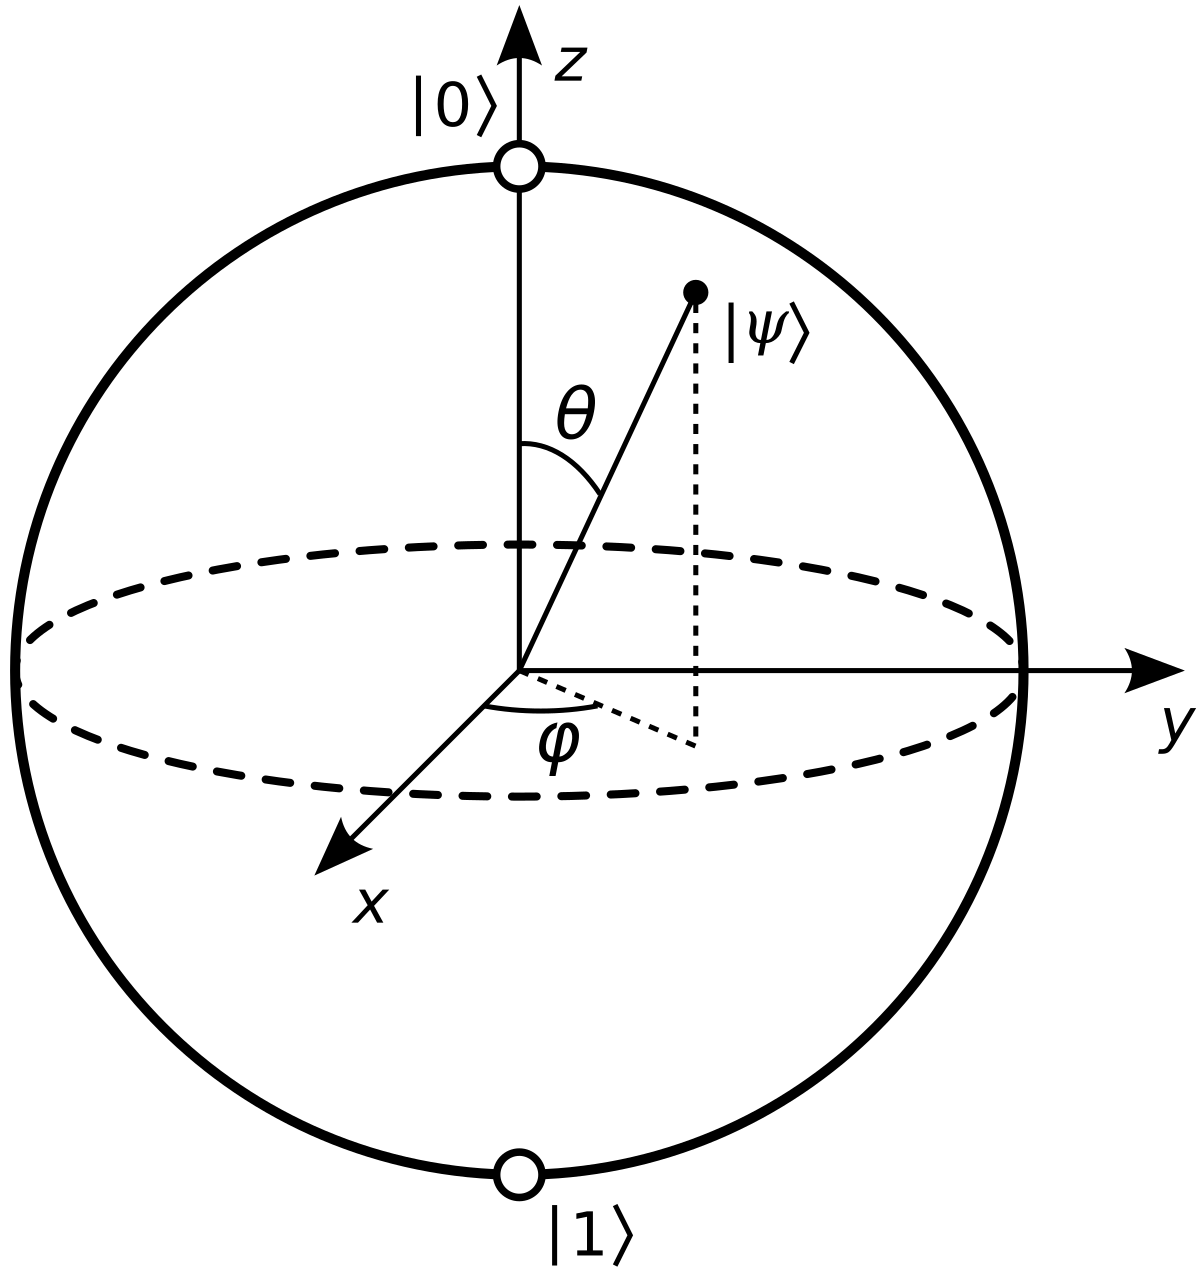
\includegraphics[width=0.4\textwidth]{Bloch_sphere}
  \caption{Sfera di Bloch}
\end{figure}
\[
  \begin{aligned}
    \ket{\psi} &= \begin{pmatrix} 
      \cos \frac{\theta }{2}\\
      e^{i \phi } \sin \frac{\theta }{2}
    \end{pmatrix} \\
    \bra{\psi} &= \begin{pmatrix} 
      \cos \frac{\theta }{2} & e^{-i \phi } \sin \frac{\theta }{2}
    \end{pmatrix}
  \end{aligned}
\] 

\subsection{Qubit}
Il Qubit codifica una quantità infinita di informazioni perchè è in sovrapposizione, ma
questo si può sfruttare soltanto all'interno del calcolo quantistico, perchè quando il
valore viene estratto si ha il collasso della funzione d'onda e potrà essere soltanto uno
dei due stati \( \ket{0} \) o \( \ket{1} \).

\vspace{1em}
\noindent
Si hanno \( n \) qubit preparati nello stato fondamentale:
\[
  \ket{\alpha_i} = \{\ket{0}, \; \ket{1}\}_i
\] 
\begin{figure}[H]
  \centering
  \begin{tikzpicture}
    \node[draw,rectangle,minimum size=1cm] (A) at (0,0) {\( \mathbb{U} \)};
    \draw[<-] (A) -- ++(-1,0) node[left] {
        \( 
        \begin{cases}
          \ket{0}_1\\
          \vdots\\
          \ket{0}_n
        \end{cases}
        \) 
      };

    \draw[->] (A) -- ++(1,0) node[right] {
        \(
        \ket{\psi } = \alpha_{1,2,\ldots,n} \ket{\alpha_1, \ldots, \alpha_n} =
        \ket{\alpha}_1 \otimes \ket{\alpha}_2 \otimes \ldots \otimes \ket{\alpha}_n
        \)
      };
  \end{tikzpicture}
  \caption{Calcolo quantistico}
\end{figure}
\noindent
Il sistema descritto da 2 qubit: $\ket{\alpha}_1 ; \ket{\alpha}_2$ si indica con:
\[
  \ket{\alpha}_1 \otimes \ket{\alpha}_2 = \ket{\alpha_1 \alpha_2} \quad \in \mathbb{C}^2 \otimes \mathbb{C}^2
\] 

\vspace{1em}
\noindent
Due qubit possono essere ad esempio 2 fotoni che possono assumere gli stati:
\[
  \begin{aligned}
    \{\ket{0}, \ket{1}\}_1\\
    \{\ket{0}, \ket{1}\}_2\\
  \end{aligned}
\] 
e quindi ci sono 4 stati possibili che formano la base. Gli stati si indicano:
\[
  \begin{aligned}
    \ket{00}\\
    \ket{01}\\
    \ket{10}\\
    \ket{11}
  \end{aligned}
\] 
Qualsiasi combinazione di questi consiste in una formazione quantistica trasportata all'interno
del circuito e quindi:
\[
  \ket{\psi} = \alpha_{00} \ket{00} + \alpha_{01} \ket{01} + \alpha_{10} \ket{10} + \alpha_{11} \ket{11}
\] 
\[
  \sum |\alpha_{ij}|^2 = 1
\] 
I coefficienti sono la probabilità di ottenere il primo stato in un certo stato fondamentale
e il secondo stato in un altro stato fondamentale.

\vspace{1em}
\noindent
Gli stati \( \ket{0} \) e \( \ket{1} \) a livello fisico hanno una differenza di energia
piccolissima, che viene annullata dal bagno termico (non si possono differenziare per
l'interferenza dell'ambiente) in cui è immerso il sistema, per
questo motivo bisogna lavorare a temperature criogeniche.
Quando un sistema fisico perde il suo stato si dice \textbf{incoerenza fisica}.

\subsubsection{Porta di Hadamard}
Il processo fisico:
\begin{figure}[H]
  \centering
  \begin{tikzpicture}
    \node[draw,rectangle,minimum size=1cm] (A) at (0,0) {\( \mathbb{U} \)};
    \draw[<-] (A) ++(-0.5,0.4) -- ++(-0.5,0);
    \draw[<-] (A) -- ++(-1,0);
    \draw[<-] (A) ++(-0.5,-0.4) -- ++(-0.5,0);

    \draw[->] (A) ++(0.5,0.4) -- ++(0.5,0);
    \draw[->] (A) -- ++(1,0);
    \draw[->] (A) ++(0.5,-0.4) -- ++(0.5,0);
  \end{tikzpicture}
  \caption{Processo fisico}
\end{figure}
\noindent
si può separare in operatori più piccoli che agiscono su un qubit, quindi sono rappresentate
da matrici unitarie \( 2 \times 2 \) (se agiscono su 2 qbit da matrici \( 4 \times 4 \)...)
in cui ogni colonna rappresenta uno stato del qubit.

\vspace{1em}
\noindent
Porta di Hadamard o porta H (non ha analogo classico):
\begin{itemize}
  \item 
    Il vettore di stato \( \ket{0} \) viene trasformato in sovrapposizione di:
    \[
      \ket{0} \to \frac{1}{\sqrt{2}} \left( \ket{0} + \ket{1} \right)
    \] 
  \item 
    Il vettore di stato \( \ket{1} \) viene trasformato in sovrapposizione di:
    \[
      \ket{1} \to \frac{1}{\sqrt{2}} \left( \ket{0} - \ket{1} \right)
    \]
\end{itemize}
\[
  \begin{aligned}
    H &= \begin{pmatrix} 
      \frac{1}{\sqrt{2}} & \frac{1}{\sqrt{2}}\\
      \frac{1}{\sqrt{2}} & -\frac{1}{\sqrt{2}}
    \end{pmatrix} \\
      &= \frac{1}{\sqrt{2}} \begin{pmatrix} 
        1 & 1\\
        1 & -1
      \end{pmatrix} 
  \end{aligned}
\] 

\vspace{1em}
\noindent
Un generico qubit viene trasformato in:
\[
  \alpha \ket{0} + \beta \ket{1} \to 
  \alpha \underbrace{\left( \frac{\ket{0} + \ket{1}}{\sqrt{2} } \right)}_{\ket{+}} +
  \beta \underbrace{\left( \frac{\ket{0} - \ket{1}}{\sqrt{2} } \right)}_{\ket{-}}
\] 
quindi torna in sovrapposizione. Si sta essenzialmente effettuando un cambiamento di base.

\section{Entanglement}
\subsection{Stato singoletto di spin}
Lo \( \ket{\text{stato "singoletto di Spin"}} \) è uno stato composto da 2 particelle
che hanno \( \text{Spin totale} = 0 \)  e spin opposto.

\vspace{1em}
\noindent
Ad esempio una sorgente
radioattiva che emette una particella in una direzione e una particella nella direzione
opposta:
\begin{figure}[H]
  \centering
  \begin{tikzpicture}
    \node[draw,circle,minimum size=1cm] (s) at (0,0) {} 
      node[below=0.5cm,align=center,scale=0.8]
      {Sorgente\\radioattiva};

    \draw[->] (s.west) -- ++(-1.5,0) 
      node[midway,above=0.1cm,draw,circle,scale=0.7] {\( p_1 \) }
      node[midway,below=0.1cm] {\( \uparrow \downarrow \) };
    \draw[->] (s.east) -- ++(1.5,0) 
      node[midway,above=0.1cm,draw,circle,scale=0.7] {\( p_2 \) }
      node[midway,below=0.1cm] {\( \downarrow \uparrow \) };
  \end{tikzpicture}
  \caption{Particelle con spin opposto}
\end{figure}
\noindent
Bisogna mantenere lo spin totale a 0, quindi se una particella ha spin "su" l'altra
deve avere spin "giù". Abbiamo 2 particelle con 2 stati e quindi 4 possibili stati:
\[
  \mathbb{C}^2 \otimes \mathbb{C}^2
\] 
Per mettere lo spin (\( \ket{0} = \text{"su"} \) e \( \ket{1} = \text{"giù"} \)) in relazione si avrà:
\[
  \ket{\text{stato "singoletto di Spin"}} =
  \frac{1}{\sqrt{2}} \left( \ket{01} - \ket{10} \right)
\] 
Le due particelle si dicono \textbf{entangled} perchè le particelle devono avere spin
opposto. Questo stato si dice \textbf{stato di Bell}.

\vspace{1em}
\noindent
Se aggiungiamo degli osservatori \( A \) e \( B \) al sistema:
\begin{figure}[H]
  \centering
  \begin{tikzpicture}
    \node[draw,circle,minimum size=1cm] (s) at (0,0) {} 
      node[below=0.5cm,align=center,scale=0.8]
      {Sorgente\\radioattiva};

    \draw[->] (s.west) -- ++(-1.5,0) 
      node[midway,above=0.1cm,draw,circle,scale=0.7] {\( p_1 \) }
      node[midway,below=0.1cm] {\( \uparrow \downarrow \) }
      node[left] (A) {\( \underset{\text{Osservatore}}{A} \) };
    \draw[->] (s.east) -- ++(1.5,0) 
      node[midway,above=0.1cm,draw,circle,scale=0.7] {\( p_2 \) }
      node[midway,below=0.1cm] {\( \downarrow \uparrow \) }
      node[right] (B) {\( \underset{\text{Osservatore}}{B} \) };
  \end{tikzpicture}
  \caption{Sistema con osservatori}
\end{figure}
\noindent
Se \( A \) fa una misura sulla particella \( p_1 \) e trova \( \ket{0} \) al \( 50\% \) e
\( \ket{1} \) al \( 50\% \). Siccome si sta lavorando in un sistema di 2 qubit, se \( A \)
trova \( \ket{0} \) esso cade nell'autostato di \( A \), ad esempio:
\begin{itemize}
  \item Al primo lancio \( A \) trova \( \ket{0}_A \) ed esso collassa nell'autostato
    \[
      \frac{1}{\sqrt{2}} \ket{01}
    \] 
    quindi \( B \) troverà \( \ket{1}_B \) al \( 100\% \)
\end{itemize}
La misura di A determina \textbf{"simultaneamente"} il valore di \( B \), senza che egli
lo abbia misurato.

\vspace{1em}
\noindent
In meccanica quantistica questa relazione è detta \textbf{correlazione di spin}
o \textbf{entanglement}. Questo avviene solo nella stessa base, se un osservatore non
conosce la base del secondo osservatore la misura rimane incerta e questa cosa è la
fondamentale per la \textbf{crittografia quantistica}.

\end{document}
